% !TeX root = ../../../main.tex
\begin{figure}[htbp]
\ChThreeFloatContents
  {ch03:fig:ite_medication}
  {\caption{Distribution of Estimated Individual Treatment Effects (ITE) for the top four medications—\textcolor{blue}{risperidone}, \textcolor{orange}{aripiprazole}, \textcolor{ChThreeForestGreen}{olanzapine}, and \textcolor{red}{haloperidol}—evaluated using different survival models and T-learner at time snapshot \(\tau=3\) month. 
  The mean treatment effect (ATE) for each medication is provided in the legend.
  (a)-(c) show T-learner ITEs for (a) CoxPH, (b) DeepSurv, (c) Random Survival Forest. 
  (d) shows the ITE for Causal Survival Forest}}
  {%
    \subfigure[\footnotesize (CoxPH, T-Learner)]{\label{ch03:fig:ite_medication_coxph}%
      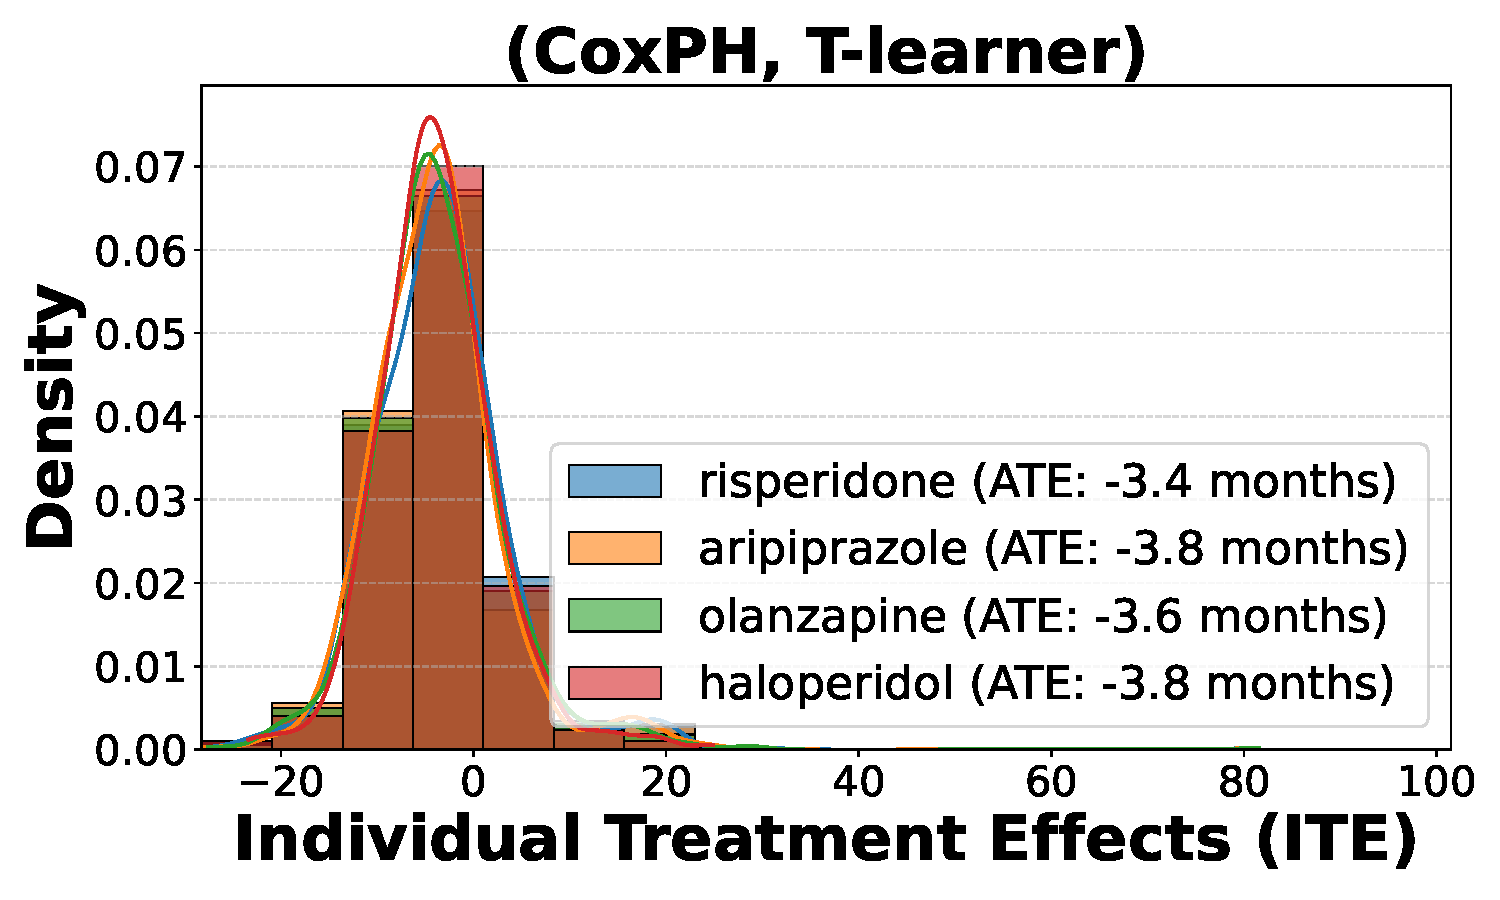
\includegraphics[width=.22\linewidth]{Appendices/appendix-ch03/images/ITE_medication/ITE_CoxPH_T-learner_med_type.pdf}}%
    \hfill
    \subfigure[\footnotesize (DeepSurv, T-Learner)]{\label{ch03:fig:ite_medication_deepsurv}%
      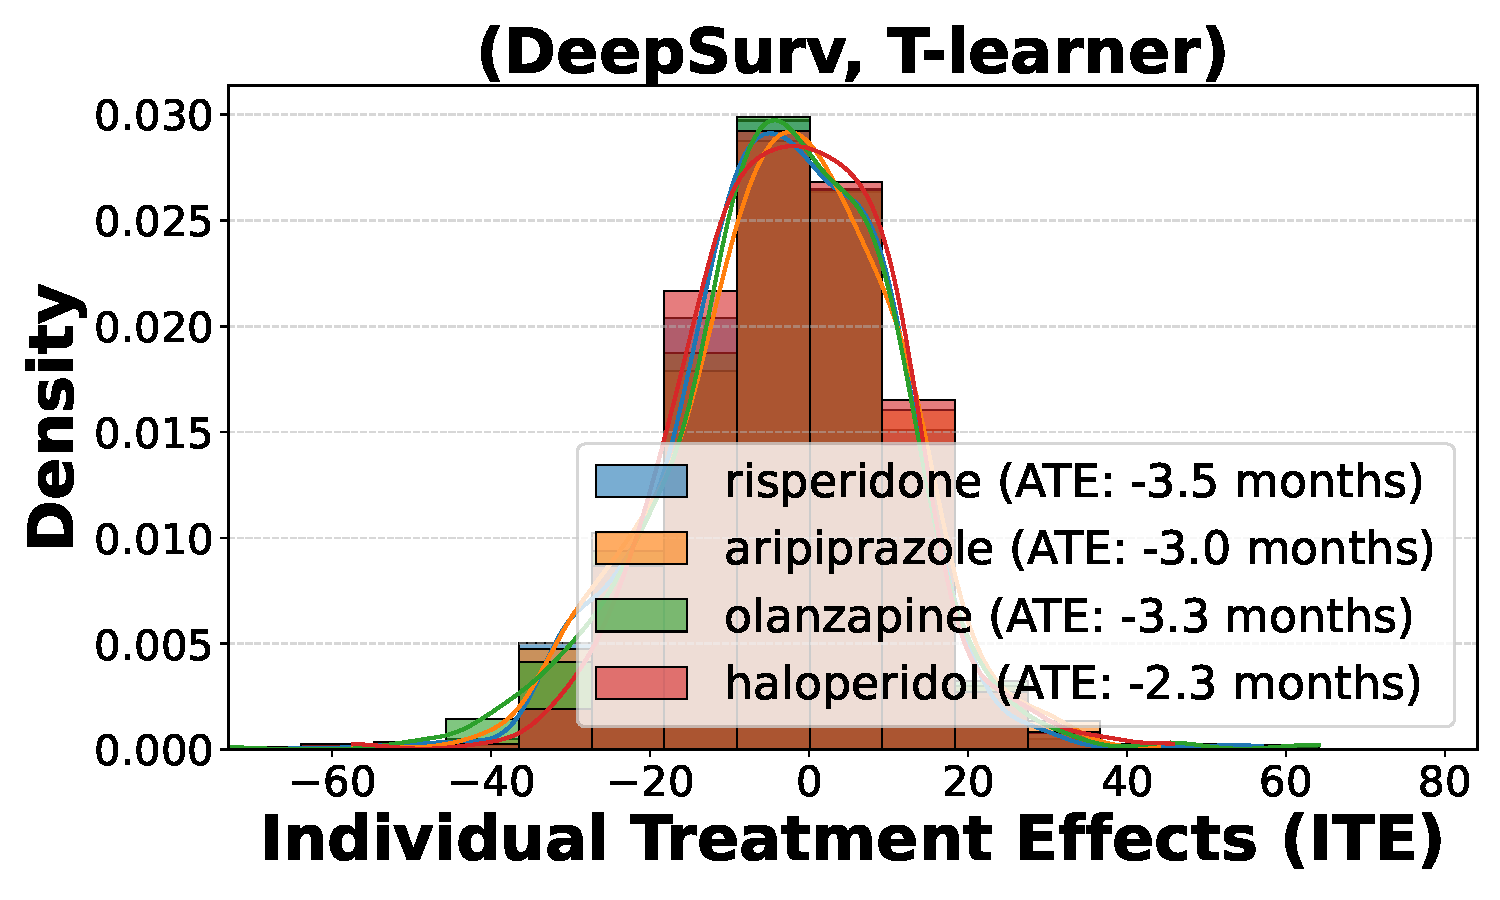
\includegraphics[width=.22\linewidth]{Appendices/appendix-ch03/images/ITE_medication/ITE_DeepSurv_T-learner_med_type.pdf}}%
    \hfill
    \subfigure[\footnotesize (RandomSurvivalForest, T-Learner)]{\label{ch03:fig:ite_medication_random_survival_forest}%
      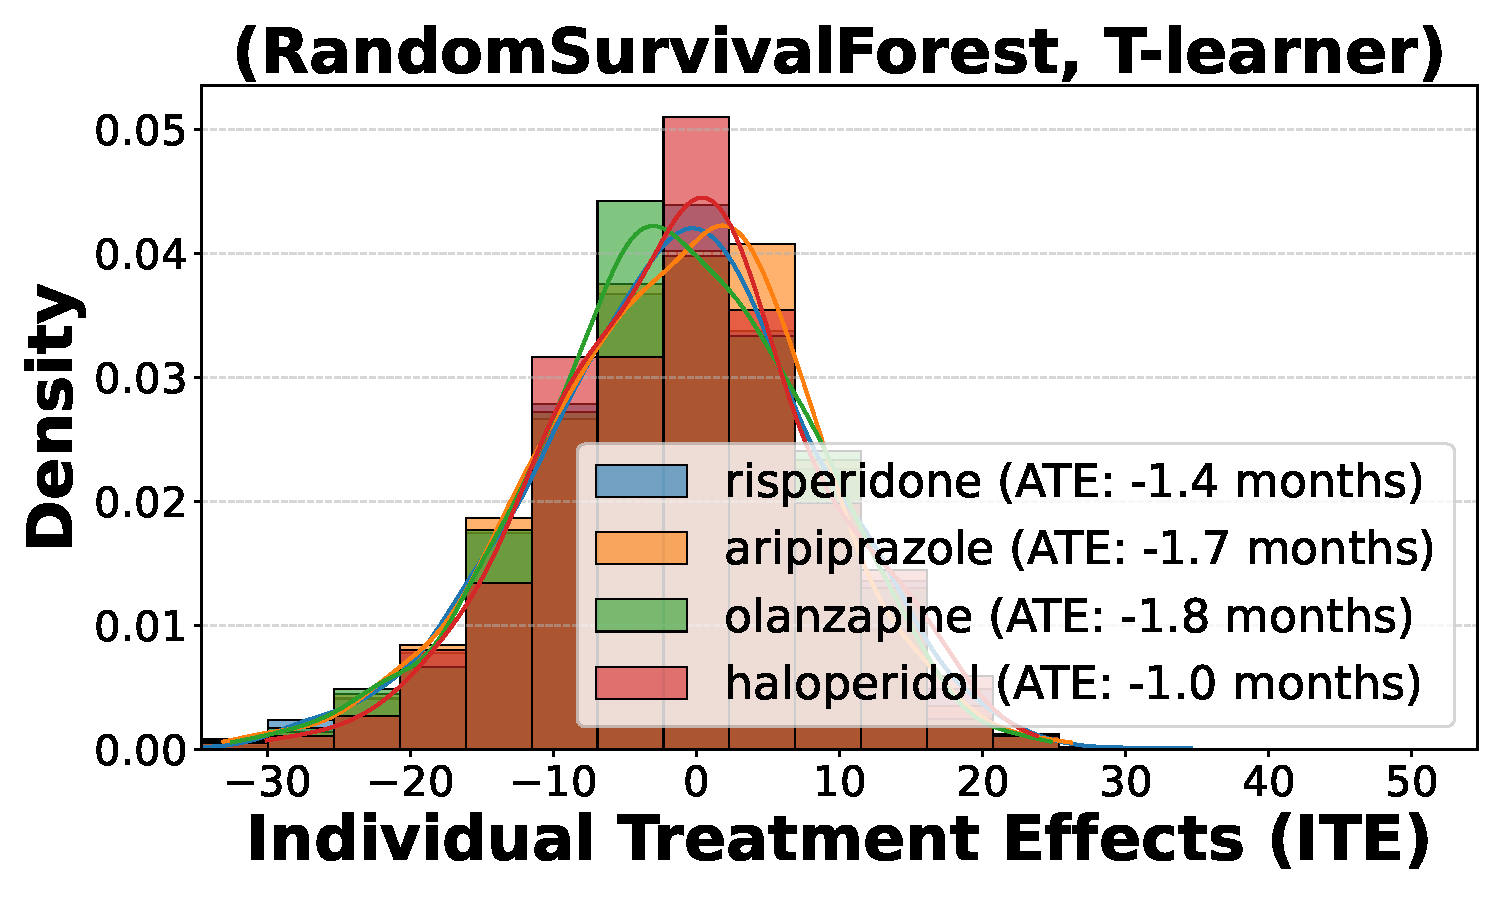
\includegraphics[width=.22\linewidth]{Appendices/appendix-ch03/images/ITE_medication/ITE_RandomSurvivalForest_T-learner_med_type.pdf}}%
    \hfill
    \subfigure[\footnotesize CausalSurvivalForest]{\label{ch03:fig:ite_medical_causal_survival_forest}%
      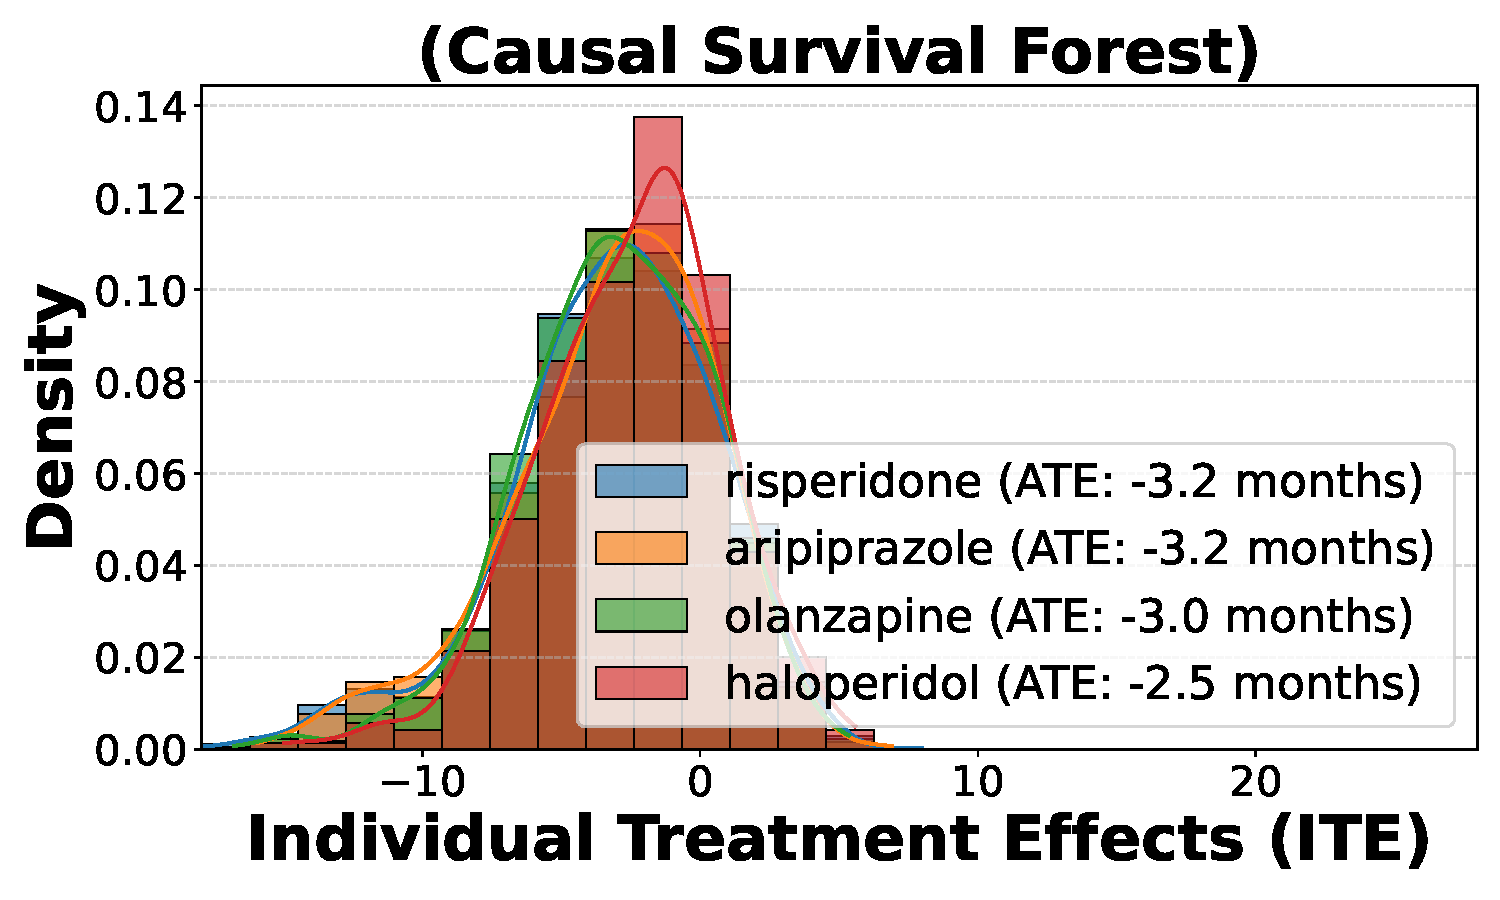
\includegraphics[width=.21\linewidth]{Appendices/appendix-ch03/images/ITE_medication/ITE_CausalSurvivalForest_Causal_Survival_Forest_med_type.pdf}}%
  }
\end{figure}